\documentclass[12pt]{beamer}
\usepackage{xcolor}
\definecolor{g1}{HTML}{70e000}
\definecolor{g2}{HTML}{9ef01a}
\usepackage{tcolorbox}
\tcbuselibrary{raster,skins}
\tcbset{frogbox/.style={enhanced,colback=g2,colframe=g1,
		enlarge top by=5.5mm,
		overlay={\foreach \x in {2cm,3.5cm} {
				\begin{scope}[shift={([xshift=\x]frame.north west)}]
					\path[draw=green!65!black,fill=green!10,line width=1mm] (0,0) arc (0:180:5mm);
					\path[fill=black] (-0.2,0) arc (0:180:1mm);
\end{scope}}}}}

\tcbset{ribbonbox/.style={enhanced,colback=g2,colframe=g1,
		fonttitle=\bfseries,
		overlay={\path[fill=blue!75!white,draw=blue,double=white!85!blue,
			preaction={opacity=0.6,fill=blue!75!white},
			line width=0.1mm,double distance=0.2mm,
			pattern=fivepointed stars,pattern color=white!75!blue]
			([xshift=-0.2mm,yshift=-1.02cm]frame.north east)
			-- ++(-1,1) -- ++(-0.5,0) -- ++(1.5,-1.5) -- cycle;}}}

\usepackage{tabularray}
\usepackage{caption}
\usepackage{subcaption}
\usepackage{tabularx}
\usepackage{graphics}
\usepackage{graphicx}
\usepackage{background}
\usepackage{tikz}
\usetikzlibrary{patterns}
\title{Intiñan.com: Discovering Peru on Horseback}
\subtitle{“Horses teach us to fly without wings and to run without fatigue.”}
%\titlegraphic{\includegraphics{\includegraphics[scale=0.2]{logo.png}}}
\titlegraphic{
\includegraphics[scale=0.2]{logo.png}}
\author{Embark on unforgettable journeys with us—your adventure starts here!}
\date{}

\setbeamertemplate{frametitle}{
	\vspace{1em} % Adjust the vertical space
	\begin{center}
		\color{black}\textbf{\insertframetitle}\\
		\vspace*{-15pt} % Make title bold and black
		\noindent\rule{\linewidth}{1pt} % Add a horizontal line
	\end{center}
}

\setbeamerfont{footnote}{size=\scriptsize} 
\setbeamertemplate{navigation symbols}{}


\begin{document}
	\begin{frame}
		\begin{center}
			{\large\textbf{\inserttitle}}\\
			\vspace*{2mm}
			{\itshape \insertsubtitle}\\
			\vspace*{2mm}
			{\inserttitlegraphic}\\
			\vspace*{2mm}
			{\textbf{\insertauthor}}
		\end{center}
	\end{frame}
	
	\begin{frame}
		\frametitle{Mission \& Vision}
%			\begin{tcbitemize}[raster columns=2,
%				colframe=g1,colback=g2,fonttitle=\bfseries, center title]
%				\tcbitem[squeezed title={Mission}]
%					{\scriptsize At Intiñan.com, our mission is to provide unforgettable horseback riding and adventure experiences that connect travelers with the rich cultural heritage and natural beauty of Cusco. We are dedicated to offering personalized, sustainable tours that allow visitors to explore lesser-known destinations while preserving the environment and supporting local communities.}
%					
%				\tcbitem[squeezed title={Vision}]
%					{\scriptsize Our vision is to become the leading horseback riding and adventure tourism agency in Peru, recognized for our deep respect for nature, our unwavering commitment to authentic cultural experiences, and our contribution to sustainable tourism. We aim to inspire a greater appreciation for Peru’s diverse landscapes, rich history, and enduring traditions through each tour.}
%			\end{tcbitemize}
				\begin{tcolorbox}[frogbox,title=Mission, fonttitle=\bfseries]
					At Intiñan.com, our mission is to provide unforgettable horseback riding and adventure experiences that connect travelers with the rich cultural heritage and natural beauty of Cusco. We are dedicated to offering personalized, sustainable tours that allow visitors to explore lesser-known destinations while preserving the environment and supporting local communities.
				\end{tcolorbox}

	\end{frame}
	
	\begin{frame}
		\begin{tcolorbox}[frogbox,title=Vision, fonttitle=\bfseries]
			Our vision is to become the leading horseback riding and adventure tourism agency in Peru, recognized for our deep respect for nature, our unwavering commitment to authentic cultural experiences, and our contribution to sustainable tourism. We aim to inspire a greater appreciation for Peru’s diverse landscapes, rich history, and enduring traditions through each tour.
		\end{tcolorbox}
	\end{frame}
	
	\begin{frame}
		\frametitle{History of the Company}
		\begin{tcolorbox}[frogbox,title=Intiñan.com,fonttitle=\bfseries]
			Founded with a passion for adventure and love for Peruvian culture, Intiñan.com was born out of a desire to offer unique horseback riding experiences that allow visitors to explore hidden gems of Cusco. Over the years, our company has evolved into a trusted provider of customized tours that showcase the rich history, breathtaking landscapes, and warm hospitality of the Andean region.
		\end{tcolorbox}
	\end{frame}
	
	
	\begin{frame}
		\frametitle{Story of the Creator}
		
		\begin{tcolorbox}[ribbonbox,title=Saturnino Pati\~no Jauja, fonttitle=\bfseries]
				I, Saturnino Patiño Jauja, grew up with a profound connection to nature and a deep appreciation for horseback riding, thanks to family traditions passed down through generations. In addition to my passion for adventure tourism, I hold a bachelor's degree in economics, specializing in data science and analysis, and I am also a skilled web developer. Inspired by a unique vision of combining adventure with cultural education, I founded Intiñan.com to share my love of horseback riding and Peru's lesser-known treasures with the world.
		\end{tcolorbox}
	\end{frame}
	
	\begin{frame}
		    \begin{tikzpicture}[remember picture,overlay]
			\node[at=(current page.center), opacity=0.2, rotate=90] {
				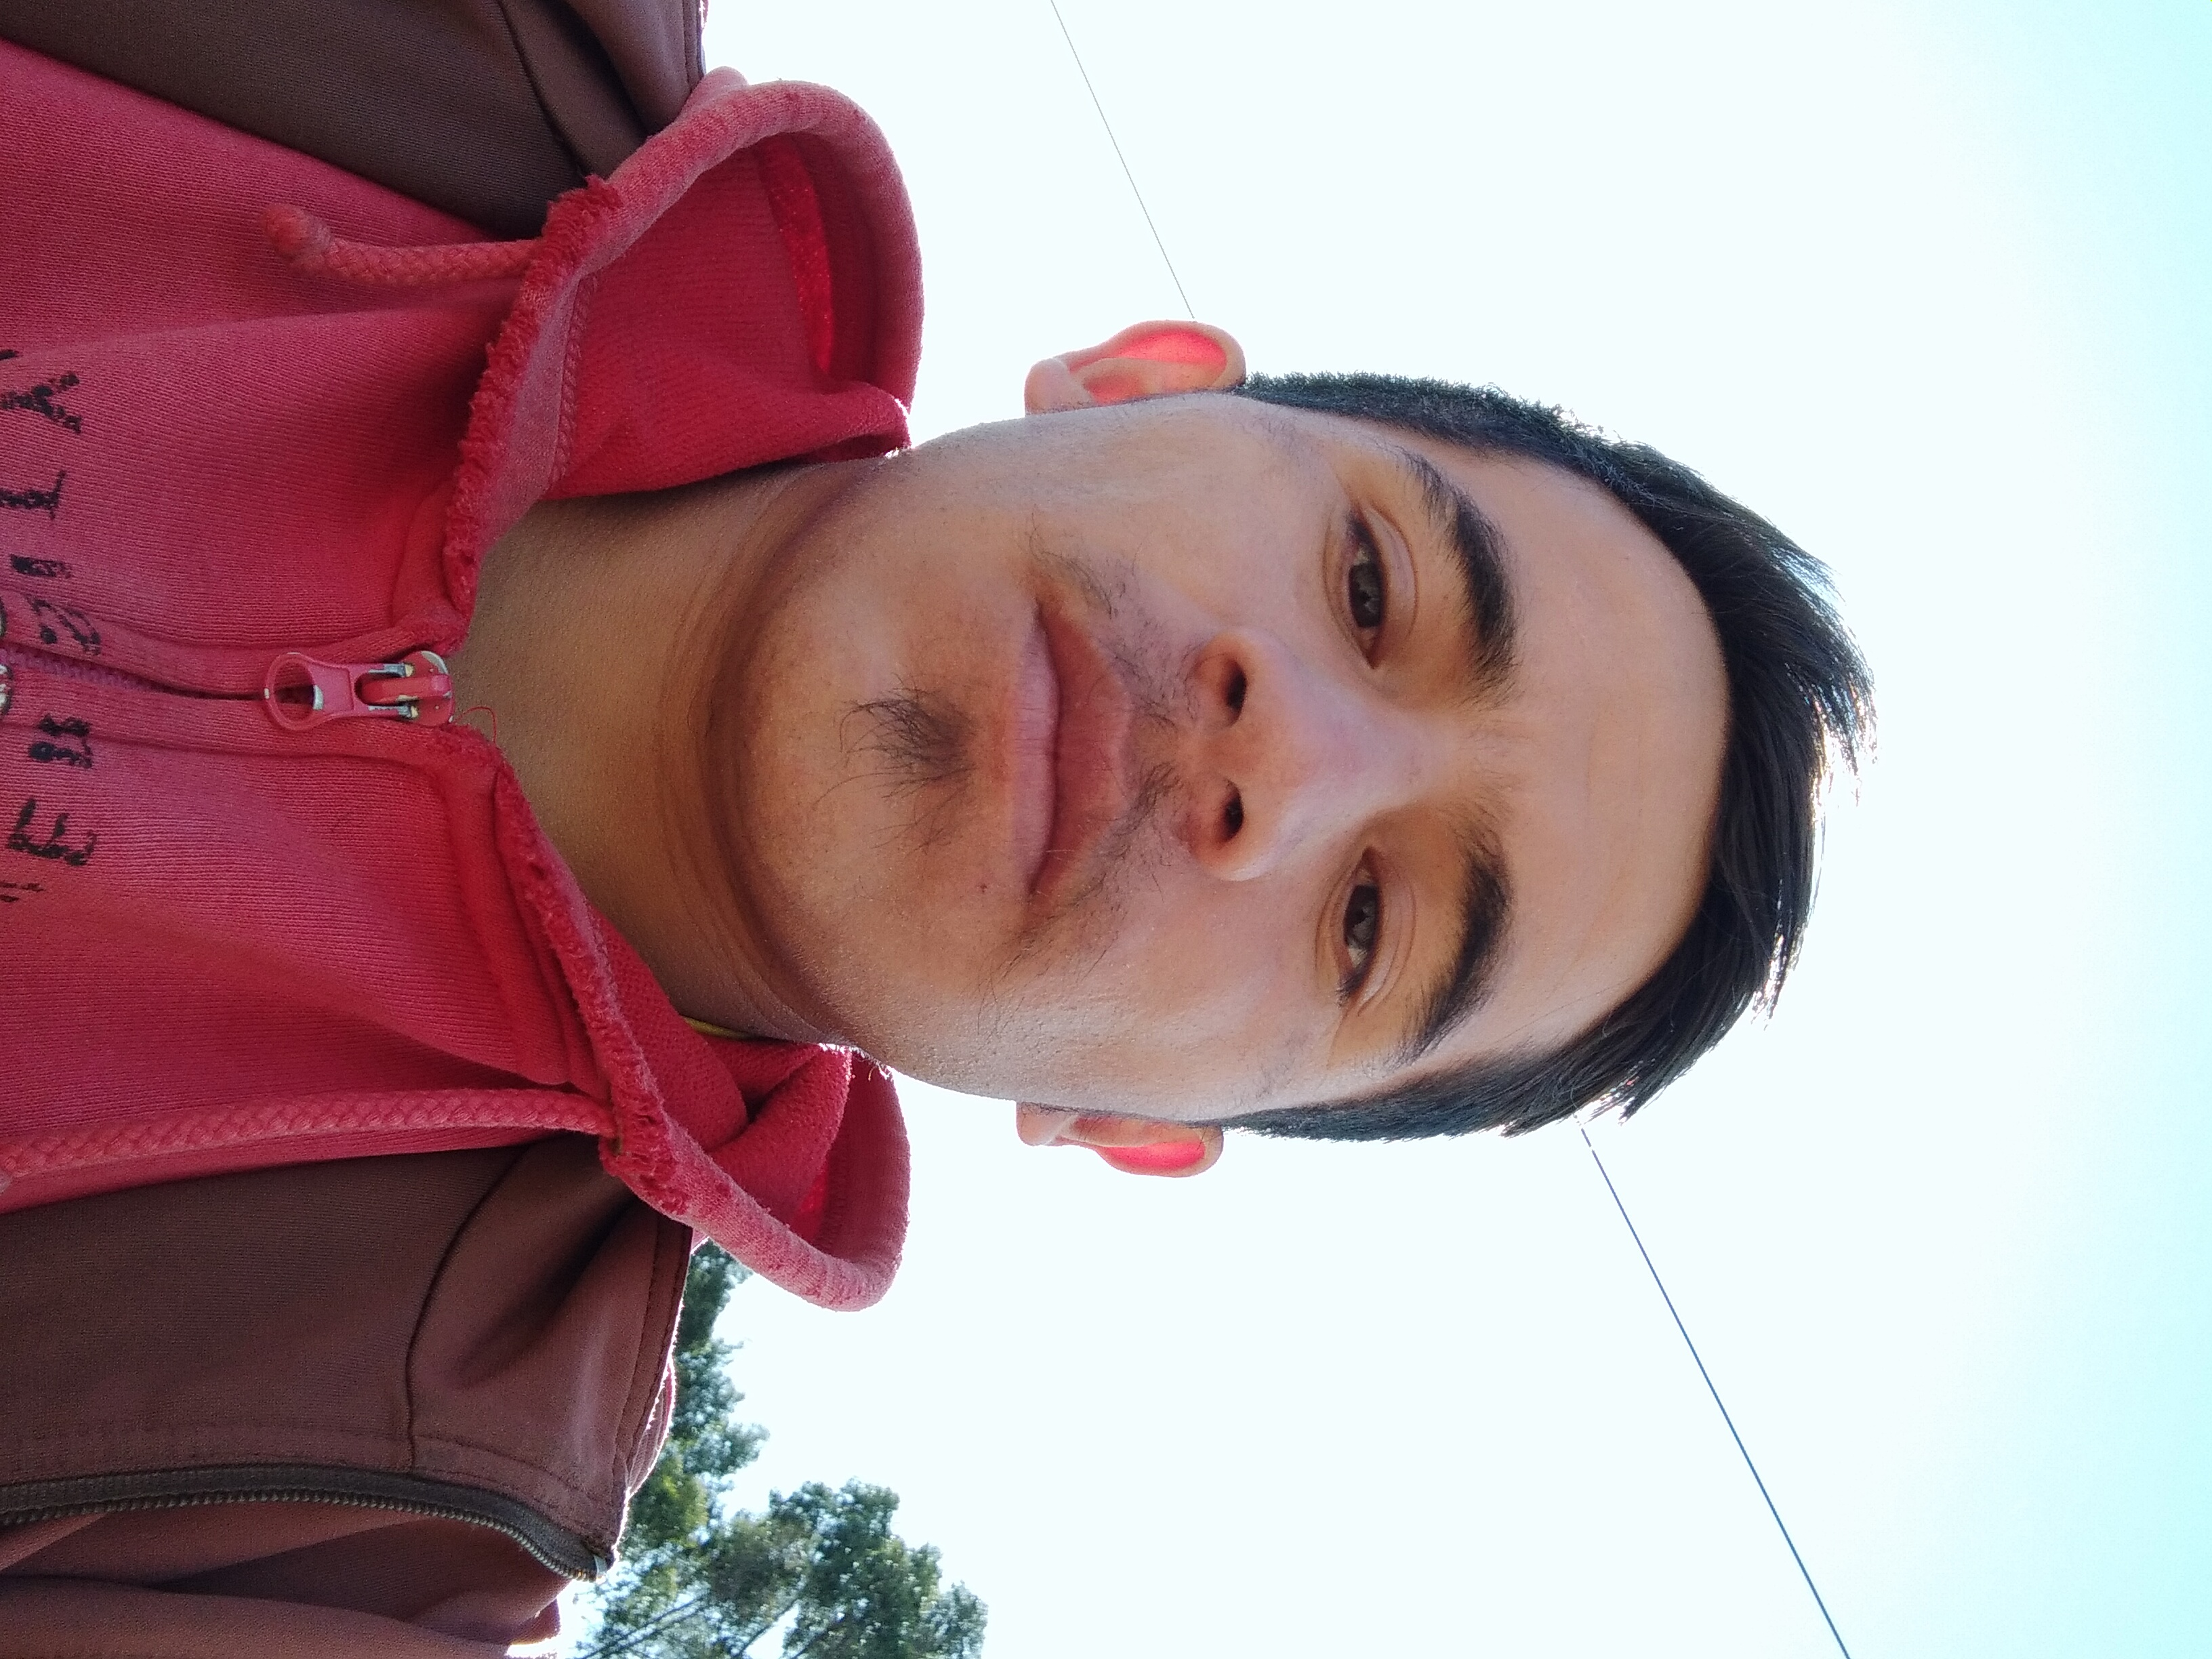
\includegraphics[width=\paperwidth, height=\paperheight]{zuco.jpg}
			};
		\end{tikzpicture}
		\centering
		\Large \textit{"Ride Through History, Embrace Nature"}
	\end{frame}	
	
\end{document}